\documentclass[tikz, border=12pt]{standalone}
\usepackage{tikz}
\usepackage{amsmath} % For \text math command
\usetikzlibrary{positioning, fit, calc, shapes.geometric, arrows.meta}

%% ── Palette ────────────────────────────────────────────────────────────────
\definecolor{clBlue}    {RGB}{219,234,254}  % process fill
\definecolor{clBlueBd}  {RGB}{ 59,130,246}  % process border
\definecolor{clOrange}  {RGB}{255,237,213}  % compute fill
\definecolor{clOrangeBd}{RGB}{234, 88, 12}  % compute border
\definecolor{clGreen}   {RGB}{220,252,231}  % update fill
\definecolor{clGreenBd} {RGB}{ 22,163, 74}  % update border
\definecolor{clRed}     {RGB}{254,226,226}  % start/skip fill
\definecolor{clRedBd}   {RGB}{220, 38, 38}  % start/skip border
\definecolor{clYellow}  {RGB}{254,249,195}  % decide fill
\definecolor{clYellowBd}{RGB}{161, 98,  7}  % decide border
\definecolor{clArrow}   {RGB}{107,114,128}  % arrows

%% ── Global styles ─────────────────────────────────────────────────────────
\tikzset{
  base/.style={
    align=center, font=\small\sffamily, thick, draw
  },
  startstop/.style={
    base, rectangle, rounded corners=12pt,
    minimum width=2.8cm, minimum height=0.9cm,
    fill=clRed, draw=clRedBd, text=clRedBd
  },
  process/.style={
    base, rectangle, rounded corners=4pt,
    minimum width=4.5cm, minimum height=1.0cm,
    fill=clBlue, draw=clBlueBd, text=clBlueBd
  },
  compute/.style={
    base, rectangle, rounded corners=4pt,
    minimum width=4.5cm, minimum height=1.0cm,
    fill=clOrange, draw=clOrangeBd, text=clOrangeBd
  },
  decide/.style={
    base, diamond, aspect=1.8,
    minimum width=3.2cm, minimum height=1.2cm,
    fill=clYellow, draw=clYellowBd, text=clYellowBd,
    inner sep=2pt
  },
  update/.style={
    base, rectangle, rounded corners=4pt,
    minimum width=4.0cm, minimum height=1.1cm,
    fill=clGreen, draw=clGreenBd, text=clGreenBd
  },
  arr/.style={
    -{Stealth[length=7pt, width=5pt]},
    thick, color=clArrow
  },
  lbl/.style={
    font=\scriptsize\sffamily, text=clArrow,
    fill=white, inner sep=2pt, rounded corners=2pt
  }
}

\begin{document}
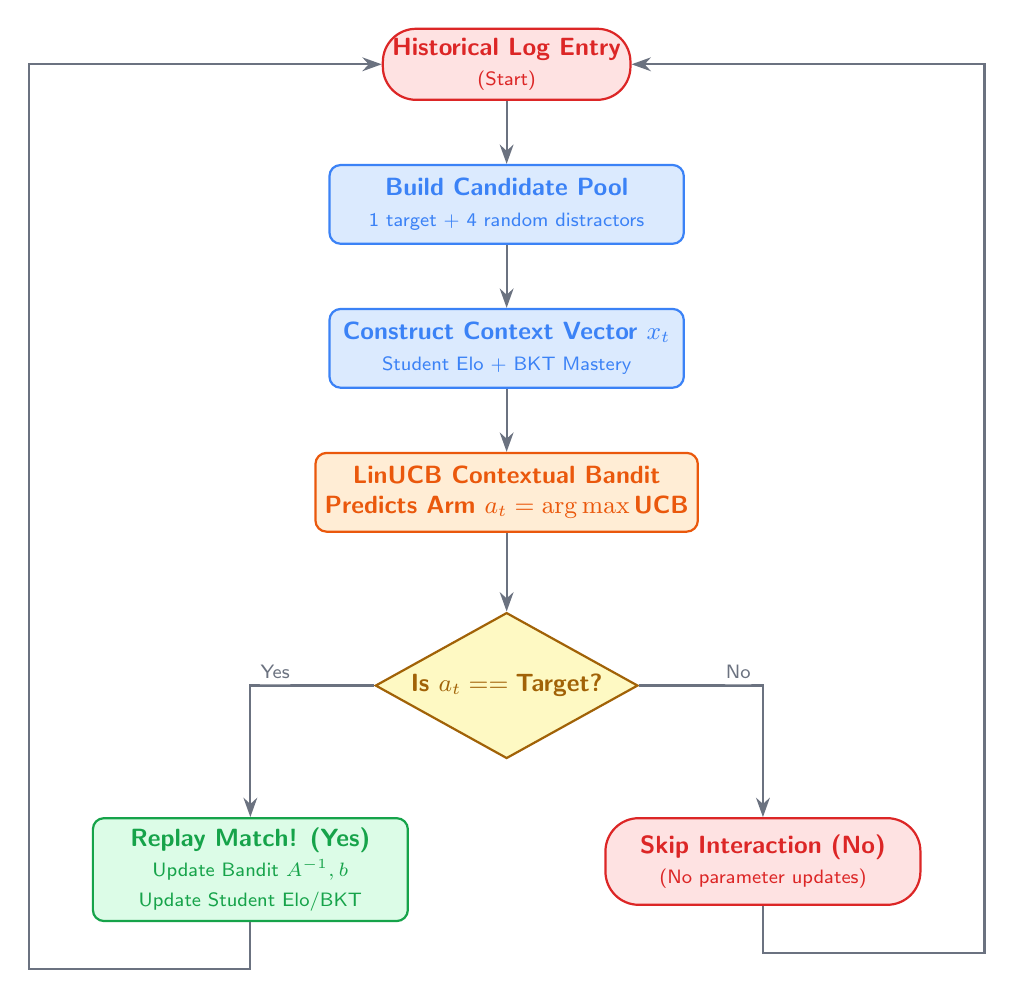
\begin{tikzpicture}[node distance=0.8cm and 1.2cm]

    % ============================================================
    % VERTICAL FLOW NODES
    % ============================================================
    \node (start) [startstop] {
      \textbf{Historical Log Entry}\\
      {\scriptsize (Start)}
    };
    
    \node (candidates) [process, below=of start] {
      \textbf{Build Candidate Pool}\\
      {\scriptsize 1 target + 4 random distractors}
    };
    
    \node (context) [process, below=of candidates] {
      \textbf{Construct Context Vector $x_t$}\\
      {\scriptsize Student Elo + BKT Mastery}
    };
    
    \node (bandit) [compute, below=of context] {
      \textbf{LinUCB Contextual Bandit}\\
      \textbf{Predicts Arm $a_t = \arg\max \text{UCB}$}
    };
    
    \node (decision) [decide, below=1.0cm of bandit] {
      \textbf{Is $a_t == \text{Target}$?}%
    };

    % ============================================================
    % BRANCHED DECISION NODES
    % ============================================================
    \node (update) [update, below left=1.2cm and 0.4cm of decision] {
      \textbf{Replay Match! (Yes)}\\
      {\scriptsize Update Bandit $A^{-1}, b$}\\
      {\scriptsize Update Student Elo/BKT}
    };
    
    \node (skip) [startstop, below right=1.2cm and 0.4cm of decision, minimum width=4.0cm, minimum height=1.1cm] {
      \textbf{Skip Interaction (No)}\\
      {\scriptsize (No parameter updates)}
    };

    % ============================================================
    % CONNECTIONS
    % ============================================================
    % Downward flow
    \draw [arr] (start) -- (candidates);
    \draw [arr] (candidates) -- (context);
    \draw [arr] (context) -- (bandit);
    \draw [arr] (bandit) -- (decision);
    
    % Branching from decision
    \draw [arr] (decision.west) -| node[lbl, above, pos=0.4] {Yes} (update.north);
    \draw [arr] (decision.east) -| node[lbl, above, pos=0.4] {No} (skip.north);
    
    % Loop back arrows going around the outside to avoid crossing nodes
    % Left feedback loop (Yes path)
    \draw [arr] (update.south) -- ++(0,-0.6) -| ($(update.west) - (0.8, 0)$) |- (start.west);
    
    % Right feedback loop (No path)
    \draw [arr] (skip.south) -- ++(0,-0.6) -| ($(skip.east) + (0.8, 0)$) |- (start.east);

\end{tikzpicture}
\end{document}
